 \documentclass[oneside,11pt]{article}


\usepackage{soul}
\usepackage{natbib}
\usepackage{hyperref}
\usepackage{bookmark}
\usepackage{graphicx}             
\graphicspath{{./Figuras/}}
\usepackage[dvipsnames]{xcolor}
\usepackage{todonotes}
\usepackage{makecell}
\usepackage[margin=1in]{geometry}
\usepackage{float}                
\usepackage{amsmath}
\usepackage{amscd}
\usepackage{amsfonts}
\usepackage{amssymb}
\usepackage{bbm}
\usepackage{booktabs}
\usepackage{nameref}
\usepackage{multirow}
\usepackage[nokeyprefix]{refstyle}
\usepackage{rotating}
\usepackage{threeparttable}
\usepackage{afterpage}
\usepackage{lscape}
\usepackage{enumerate}
\usepackage{caption}
\usepackage{subcaption}
\usepackage{epstopdf}
\usepackage{setspace}
\usepackage{svg}
\usepackage{dsfont}
\usepackage{amsthm}
\usepackage{tocloft}
\usepackage{etoc}
\usepackage{lmodern}
\usepackage{bm}
\usepackage[T1]{fontenc}
\usepackage{tgpagella}

\epstopdfDeclareGraphicsRule{.tiff}{png}{.png}{convert #1 \OutputFile}
\AppendGraphicsExtensions{.tiff}

\epstopdfDeclareGraphicsRule{.tif}{png}{.png}{convert #1 \OutputFile}
\AppendGraphicsExtensions{.tif}

\def\sym#1{\ifmmode^{#1}\else\(^{#1}\)\fi}

\usepackage{tikz}
\usetikzlibrary{shapes.geometric, arrows}
\usetikzlibrary{calc}
\usetikzlibrary{matrix}

\tikzset{ 
    table/.style={
        matrix of nodes,
        row sep=-\pgflinewidth,
        column sep=-\pgflinewidth,
        nodes={
            rectangle,
            draw=black,
            align=center
        },
        minimum height=1.5em,
        text depth=0.5ex,
        text height=2ex,
        nodes in empty cells,
%%
        every even row/.style={
            nodes={fill=gray!20}
        },
        column 1/.style={
            nodes={text width=2em,font=\bfseries}
        },
        row 1/.style={
            nodes={
                fill=black,
                text=white,
                font=\bfseries
            }
        }
    }
}


\usepackage{colortbl}
\usepackage{url}
\urlstyle{rm}
\definecolor{darkblue}{rgb}{0,0,.4}
\hypersetup{colorlinks=true, breaklinks=true, citecolor=Maroon, linkcolor=darkblue, menucolor=darkblue, urlcolor=darkblue}

\newtheorem{theorem}{Theorem}
\newtheorem{claim}[theorem]{Claim}
\newtheorem{prop}[theorem]{Proposition} 
\newtheorem{cor}[theorem]{Corollary} 
\newtheorem{assumption}{Assumption} 
\newtheorem{lem}{Lemma} 

\DeclareRobustCommand{\hlgr}[1]{{\sethlcolor{green}\hl{#1}}}


\usepackage{comment}
%para esconder columnas en tablas (enrique)
\usepackage{array}
\newcolumntype{H}{>{\setbox0=\hbox\bgroup}c<{\egroup}@{}}
\linespread{1.25}

\newcommand{\wh}{\widehat}
\usepackage{anyfontsize}

\usepackage[linesnumbered,vlined,ruled,commentsnumbered]{algorithm2e}

\DontPrintSemicolon
\newcommand{\To}{\mbox{\upshape\bfseries to}}
\newcommand{\E}{\mathbb{E}}

\DeclareCaptionFormat{cont}{#1 (cont.)#2#3\par}
%%% HELPER CODE FOR DEALING WITH EXTERNAL REFERENCES
\usepackage{xr}
\makeatletter
\newcommand*{\addFileDependency}[1]{
  \typeout{(#1)}
  \@addtofilelist{#1}
  \IfFileExists{#1}{}{\typeout{No file #1.}}
}
\makeatother


\newcommand*{\myexternaldocument}[1]{
    \externaldocument{#1}
    \addFileDependency{#1.tex}
    \addFileDependency{#1.aux}
}

%\myexternaldocument{OA}

%%%%%%%%%%%%%%%%%%%%%%%%%%%%%%%% DOCUMENT
\begin{document}

\title{IMSS RPCI \thanks{We want to thank.}}
\author{Marco Medina \and Eduardo Alcaraz \and Gabriela López \and Luis Martínez \and Enrique Seira  \and Christopher Woodruff\thanks{Seira: MSU, seiraenr@msu.edu (corresponding author); Alcaraz: IMSS, eduardo.alcarazp@imss.gob.mx; López: IMSS, ; Martínez: IMSS, luis.martinezch@imss.gob.mx; Medina:  ITAM, marco.medina@itam.mx}}
\date{This draft:  \today \\[2 cm]}

%\vspace{.5in}


\maketitle
\thispagestyle{empty}
\begin{abstract}

%Abstract here. 

\end{abstract}

\vspace{.3in}

\textbf{Keywords: }

\textbf{JEL codes:}

\newpage

\pagenumbering{arabic}
\etocdepthtag.toc{mtchapter}
\etocsettagdepth{mtchapter}{subsection}
\etocsettagdepth{mtappendix}{none}

\section{Introduction} \label{introduction}

According to the International Labour Organization, close to 60 percent of workers worldwide work in the informal sector \citep{ILO_2018}. The informal sector comprises close to a third of economic activity in developing countries, twice as much as in developed ones.\footnote{\url{https://www.imf.org/external/pubs/ft/fandd/2020/12/pdf/what-is-the-informal-economy-basics.pdf}} The prevalence of informality may not be innocuous. Informality facilitates tax evasion, weakening state capacity. Moreover, having some workers and not others be subject to taxes could cause distortions in the allocation of resources, lowering income \citep{Misallocation}. 

In this paper, we focus on informality in the labor market. Payroll tax evasion occurs along several margins. First, firms may not register with the tax authority. Second, even if the firm is registered, they may hire workers and not report them to the social security administration (IMSS), this avoids paying a 24\% payroll tax. These two margins are the focus of \cite{Ulyssea}. A third understudied margin revolves around what wage to declare to tax authorities when both the firm and the worker are registered with tax authorities. Income and payroll taxes create incentives for both firms and workers to report lower salaries. 
\cite{kumler2020enlisting} note that ``having firms report employees’ wages is no guarantee of accurate reporting in a low-enforcement context like Mexico.'' Being registered with IMSS is mandated by law. Workers have an interest in being registered as it gives them access to free medical services, provides them with disability insurance, and contributes a proportion of the wage to a personal retirement savings account, as we explain in detail below. While the disability insurance and the amount deposited in the worker's retirement account are an increasing function of the reported wage, access to medical services is not.

\cite{kumler2020enlisting} estimate that the median under-reporting of wages in Mexico is close to 30\% for small firms and 56\% for large ones. They also find that a regulatory change that (a) tied the wage reported more closely and positively with retirement savings and (b) increased wage transparency to the worker, increased wages reported to IMSS, especially for the younger cohorts which were more likely affected by the regulatory change. %Unfortunately, because the reform involved both changes in the benefits and changes in the information provided to workers about the wage reported by their employer, it is not possible to attribute causality among these two. 
It is difficult to know what aspect of the reform ---wage transparency or incentives to report wages--- is driving the main finding.\footnote{It is also possible that because the treatment-control comparisons involve comparing older versus younger workers, the differences in differences results could be driven by differential time trends. The reform was implemented just after the tequila crisis, a time of macroeconomic upheaval.} One the one hand workers can be misinformed and erroneously assume that they are formally registered when in fact they are not. On the other hand, given that workers could collude with the employer on what wage to report, incur fewer taxes, and split the tax savings. \cite{kumler2020enlisting} note that the  ``extent workers are aware of underreporting by their employers and, relatedly, to what extent the effects of the pension reform we observe are due to the change in incentives versus the change in information'' are two open questions.  

To investigate this IMSS conducted a brief survey by email covering more than 200,000 IMSS registered workers. We found that only $66.5\%$ think their employer reports the complete wage to IMSS, with $10.2\%$ saying the employer definitely does not, and $23.3\%$ claiming they don't know. Interestingly almost 1 in 5 say they explicitly discussed with their employer which wage to report to IMSS. Taken literally, this suggests that part of the misreporting is collusive and workers are likely informed about it, but maybe not a large part. If workers were fully informed we would expect that providing them with information about their formal status and wage would have no effects. 

This paper estimates the causal effect of providing information to workers about whether their employer has registered them with IMSS and the wage that is registered. Using the methodology of \cite{deChaisemartin2022} we estimate the effect of this information on the worker's registered wage and on job termination by exploiting staggered adoption of RPCI (\textit{Reporte Personalizado de Cotizaciones en el IMSS}). The RPCI App gives workers a low-cost way to check their formal status in the extensive (begin registered) and intensive margin (how many days of work were registered and at which wage level). Before RPCI workers had to ask for an appointment to an IMSS office, show IDs, and wait your turn to get the information. This could take weeks of delay and hours of waiting in line. In interviews with IMSS officials they estimate that less than \hl{XX\%} of workers did it.\footnote{\url{https://www.youtube.com/watch?v=phKa31-QH4M}.}

We show that, before adoption, early and late RPCI adopters had similar time trends of wages and employment status, but wages steadily increase exactly when the RPCI App is downloaded, reaching an average increase of 20 pesos 1 year after (close to 5\% of mean wages). While there is an increase in the intensive margin, we detect no effect on the extensive margin, i.e. on the likelihood of being registered at IMSS. We find that the effect is larger for males, older workers (55 to 65), and for those earning 1 to 3 minimum wages, firms that registered agriculture and construction as their industry, and small firms (<50 workers).

We implemented an RCT to vary 






%By comparing the salaries reported by firms in groups of characteristics in survey versus in Social Security data \cite{kumler2020enlisting} show average underreporting of wages to IMSS, 

\section{Context} \label{context}

The Instituto Mexicano del Seguro Social (IMSS) is the Mexican social security agency. Workers in Mexico with formal jobs are registered by their employer to the IMSS, which combines giving access to medical services as well as administering resources for the retirement of affiliated workers. IMSS benefits encompass several areas, including occupational risk insurance, maternity insurance, disability schemes, pensions, among others.

Employers report to the IMSS the worker's job status, such as wage earned, days worked, etc. Taxes and employer's social security contributions are proportional to the reported wage. Employers may underreport the actual wage earned by the worker \citep{kumler2020enlisting}. Underreporting wages can be detrimental to the worker, since social security, retirement and pension benefits also depend on the reported wage. Workers tend to discover wage underreporting until they are about to retire, when they ask for their report on quoted weeks (quoted weeks are the period of time quoted by the worker with the IMSS). The report contains the information for each job the worker has been registered for at the IMSS, including wages, employers' firm name, and tenure. Since they ask for the report when they are about to retire, there isn't much they can do if they find underreporting. With this in mind, IMSS created the RPCI, a personalized report on the worker's current job, which includes information on the worker's current reported wage and employer's legal name.\footnote{Figure \ref{rpci_example} shows a screenshot of the IMSS app and an example of the RPCI's PDF workers receive.} The objective is to make access to information on the worker's register easier, and increase compliance via enforcement from the workers.

We conducted an online survey of workers enrolled at IMSS during August 2021. The survey was sent via email to a random sample of workers. Figure \ref{fig:hist_knowledge_register_survey} shows the answers to some of the survey questions, related to knowledge about IMSS and wage reporting to the IMSS. This survey and our findings serve as motivation for this paper.

We find that not all workers know the status of their enrollment in the IMSS. Even though all workers were actually enrolled at IMSS, $1.5\%$ of workers said they weren't enrolled, and $4\%$ said they didn't know if they were enrolled. Moreover, workers don't always know their reported wage or know the existence of wage underreporting by their employer. When we asked in the survey if their employer reported their complete wage to the IMSS, $23.3\%$ answered that they didn't know, and $10.2\%$ said no. Most workers don't talk with their employers about which wage will be reported to the IMSS. $81\%$ of workers say they didn't talk with their employer about which wage to report to the IMSS. On the other hand, workers are aware that their benefits depend on the reported salary. $88.9\%$ report being aware that part of their reported wage goes to their savings accounts. $83.7\%$ report being aware of the existence of an accident insurance when being enrolled at IMSS, that is proportional to their reported wage.

Wage underreporting happens at different extents, and some workers are aware of its occurrence. Workers, in fact, could agree to underreport their own wage if the gains of paying fewer taxes are given to them and are more valued than the benefits obtained at the IMSS. If underreporting was part of an agreement, receiving information about my current job would not have an effect on me since I already knew this information. The survey answers don't exactly reflect this story. Most workers don't talk with their employers about their wages, and many don't know if their complete wage is reported. With this in mind, if under reporting happened, receiving information about my current job enrollment could trigger workers to force higher compliance in wage reporting from their employees.

\section{Data} \label{data}

We use administrative data on workers' records from IMSS. For our main analysis, we use a monthly panel dataset for a random sample of workers registered at IMSS during January 2021, one month before the RPCI launch. The dataset follows the workers from January 2018 to February 2022. It includes variables on the workers' registration, such as their wage, industry, age group, firm, job modality, and state. It also contains a variable on when the worker registers for the RPCI. We will refer to this dataset as the worker panel data.

Apart from the administrative data, we have data obtained through the survey we conducted via email. We received 233,709 responses from workers who answered the survey. We will refer to this dataset as the survey data. The survey included questions on the wage the worker earns and the wage the worker thinks is registered at IMSS. It also includes questions to test the worker's level of knowledge about IMSS. This allows us to investigate the level of knowledge workers have about their reported wages. We will refer to this dataset as the survey data.

\section{Specification} \label{specification}

Our main analysis is performed using panel data. The treatment in our context is registration for the RPCI, which is a staggered treatment. Workers can register for the RPCI at any time following the launch, and they have access to their personalized reports every month after registration. As a result, we observe treatment cohorts.

To evaluate the causal treatment effect of registering for the RPCI, we conduct a difference-in-difference analysis. Recent literature (\citealt{callaway2021difference}; \citealt{sun2021estimating}; \citealt{de2020two}) shows that using two-way fixed effects estimates can be misleading or biased, as the estimate can be a weighted average of the ATEs where some of the weights are negative or forbidden comparisons are made under not-so-rare cases, such as heterogeneous treatment effects across treatment cohorts over time. Several authors have proposed alternative specifications to address this issue. We use the specification proposed by \cite{de2020two}, with the robust dynamic option to account for possible heterogeneous treatment effects across cohorts.

\section{Results} \label{results}

We examine the effect of registering for the RPCI on enrollment and wages. The RPCI provides information about the worker's current enrollment at IMSS. If the worker's current job information is correct, receiving a report on it should not have an effect on their reported wage or employment status compared to those who didn't register for the RPCI. The worker panel data allows us to determine whether a worker $i$ was enrolled at IMSS during period $t$ and at what wage they were enrolled. We create a dummy variable, \textit{Enrolled}, where 1 indicates the worker was enrolled at IMSS during a given period. We also have information on the workers' reported wages, but this is conditional on them being enrolled at IMSS during a given period. If a worker is discharged, we don't observe their wage and have a missing value for this variable. If registering for the RPCI has an effect on the probability of being enrolled (the extensive margin), the effect on reported wages could be biased. To address this, we create another variable, \textit{Formal Wage}, which is well-defined for all periods. It is the same as the reported wage, except it is 0 instead of a missing value if the worker isn't enrolled at IMSS during a given period.

Table \ref{tab:dcdh_rpci} presents the estimates obtained with the \cite{de2020two} specification. We find no effect on the probability of being enrolled at IMSS. We observe a positive and significant treatment effect of registering for the RPCI on the reported wage, but no significant effect on formal wages. This could be due to the imputation of zeros to formal wages, which would lower the average treatment effect. Figure \ref{fig:event_study_rpci} presents the event studies using the \cite{de2020two} specification. The event study shows no differences between treated and control groups before registering for the RPCI. The event studies demonstrate a positive effect of registering for the RPCI on the worker's registered wage.

We also investigate the heterogeneity of treatment effects by worker and firm characteristics. Figure \ref{fig:heterogeneity_worker_rpci} shows the resulting estimated coefficients by worker characteristics. When examining gender, we can observe a higher treatment effect on men's wages. Young workers (25-35 years) have a significant positive treatment on formal wages. Older workers near retirement age (65 years) have interesting treatment effects: a negative treatment effect on the probability of being enrolled, a negative treatment effect on formal wages, but a positive treatment effect on reported wages. These results could indicate that older workers have a make-or-break negotiation with their employers when they find out their actual reported wage to IMSS, as their pension or savings depend on the reported wage. We also observe a positive treatment effect for workers earning between 1 and 2 minimum wages and those earning between 2 and 3 minimum wages, while there is no effect for those with higher wages. This is consistent with firms mostly underreporting wages, reporting just the minimum wage to IMSS.

Figure \ref{fig:heterogeneity_firm_rpci} shows the resulting estimated coefficients by firm characteristics. Job registers at IMSS have a municipality identifier when they are permanent jobs registered by a firm. We examine the treatment effect for workers in the MX-USA border and workers away from the border. We use INEGI's definition of border municipalities, which is the same as that used to establish differentiated minimum wages between the border and the rest of the country. We find a positive treatment effect on wages for both workers along the border and away from the border. By region, we find a positive treatment effect on wages in the Central-West and North region, with the effect being higher for the former. By firm industry, we find positive treatment effects on wages in the agriculture, construction, and services industries. By firm size, we find a positive treatment effect on small firms (2-5 workers) and medium firms (6-50 and 51-250 workers).

\section{Conclusion} \label{conclusion}

%%%%%%%%%%%%%%%%%%%%%%%%%%%%%%%%%%%%%%%%%%%%%%%%%%%%%%%%%%%%%

\newpage

%%%%%%%%%%%%%%%%%%%%%%%%%%%%%%%%%%%%%%%%%%%%%%%%%%%%%%%%%%%%%
%BIBLIOGRAPHY

\clearpage
\bibliographystyle{ecta}
%\bibliographystyle{authordate1}
%\bibliographystyle{amsalpha}
%\bibliographystyle{AEA}

\bibliography{References}

%\FloatBarrier
%%%%%%%%%%%%%%%%%%%%%%%%%%%%%%%%%%%%%%%%

\clearpage
\singlespacing

\section{Tables}


\begin{table}[H]
\footnotesize
\centering
\begin{threeparttable}
\centering
\caption{Summary Statistics\label{tab:summary_stats_rpci}}
%\textit{Do file: summary_stats_rpci.do}

\begin{tabular}[t]{@{}l}
\toprule
\toprule
\begin{tabular}[t]{lccc}
\input 03_Tables/muestra_10porciento/summary_stats_rpci
\midrule
Workers & & & 1,412,210\\
Firms & & & 339,884\\
\end{tabular}

\tabularnewline 
\bottomrule
\bottomrule

\end{tabular}

\begin{tablenotes}
\setlength\labelsep{0pt}
\scriptsize
\item \textit{Notes}: This table shows summary statistics on selected variables for our final sample. \textit{Sample:} Panel data for a random sample of the workers enrolled at the Mexican Institute of Social Security (IMSS) during 2020 and January 2021 (before the RPCI launch). \textit{Registered for RPCI} is a dummy where 1 means worker $i$ registered for the RPCI at some point in our sample. \textit{Enrolled} is a dummy variable where 1 means worker $i$ was enrolled at IMSS during period $t$. \textit{Women}, \textit{Outsourcing} and \textit{Eventual} are dummies where 1 means worker $i$ is a woman, an outsourced worker or an eventual worker, respectively. \textit{Wage} is registered wage for worker $i$ during period $t$. \textit{N} is the number of non-missing observations for each variable. Wage and worker characteristics are only available if the worker was registered during period $t$. \textit{Workers} and \textit{Firms} are the number of unique workers and firms in our sample. This table is referenced in %\hyperref[subsec:workers]{Section} \ref{subsec:workers}.
\end{tablenotes}
\end{threeparttable}
\end{table}

\clearpage


\begin{table}[H]
\footnotesize
\centering
\begin{threeparttable}
\centering
\caption{RPCI effect on enrollment and wages\label{tab:dcdh_rpci}}
%\textit{Do file: event_study_rpci.do}

\begin{tabularx}{0.75\textwidth}[t]{@{}l@{}l@{}l}
\toprule
\toprule
\begin{tabular}[t]{p{0.2\textwidth}P{0.15\textwidth}}
& Enrolled \\
\midrule
\input 03_Tables/muestra_10porciento/dcdh_alta
\end{tabular}
&
\begin{tabular}[t]{HP{0.15\textwidth}}
& Formal Wage \\
\midrule
\input 03_Tables/muestra_10porciento/dcdh_sal_formal
\end{tabular}
&
\begin{tabular}[t]{HP{0.15\textwidth}}
& Wage$^\dagger$ \\
\midrule
\input 03_Tables/muestra_10porciento/dcdh_sal_cierre
\end{tabular}

\tabularnewline 
\bottomrule
\bottomrule

\end{tabularx}

\begin{tablenotes}
\setlength\labelsep{0pt}
\scriptsize
\item \textit{Notes}: This table shows the effect of registering to the RPCI on enrollment and the worker's wage. \textit{Sample:} Panel data for a random sample of the workers enrolled at the Mexican Institute of Social Security (IMSS) during during 2020 and January 2021 (before the RPCI launch). \textit{Enrolled} is a dummy variable where 1 means worker $i$ was enrolled at IMSS during period $t$. $\dagger$ \textit{Formal Wage} and \textit{Wage} are the registered wage for worker $i$ during period $t$, the difference is \textit{Formal Wage} is 0 when the worker isn't enrolled, while \textit{Wage} is missing when the worker isn't enrolled. The coefficient displayed is the average treatment effect estimated following \cite{de2020two}, using the robust dynamic option to account for possible heterogeneous treatment effects across cohorts. The number of observations are the number of differences of the outcome and of the treatment used in the estimation. The effect is the average effect of the treatment across the switchers. Switchers is the number of switchers this effect applies to. Robust standard errors clustered by worker id in parenthesis. *** $p<0.01$, ** $p<0.05$, * $p<0.1$. This table is referenced in %\hyperref[subsec:workers]{Section} \ref{subsec:workers}.
\end{tablenotes}
\end{threeparttable}
\end{table}

\clearpage


\begin{comment}
\subsection{RPCI effect on wage changes}

\begin{table}[H]
\footnotesize
\centering
\begin{threeparttable}
\centering
\caption{RPCI effect on wage changes\label{tab:dcdh_wage_changes_rpci}}
%\textit{Do file: yearly_volatility_rpci.do}

\begin{tabularx}{0.75\textwidth}[t]{@{}l@{}l@{}l}
\toprule
\toprule
\begin{tabular}[t]{p{0.2\textwidth}P{0.15\textwidth}}
& Wage Changes \\
\midrule
\input 03_Tables/muestra_10porciento/dcdh_sal_diff_yr
\end{tabular}
&
\begin{tabular}[t]{HP{0.15\textwidth}}
& Wage Raises \\
\midrule
\input 03_Tables/muestra_10porciento/dcdh_sal_mayor_yr
\end{tabular}
&
\begin{tabular}[t]{HP{0.15\textwidth}}
& Wage Cuts \\
\midrule
\input 03_Tables/muestra_10porciento/dcdh_sal_menor_yr
\end{tabular}

\tabularnewline 
\bottomrule
\bottomrule

\end{tabularx}

\begin{tablenotes}
\setlength\labelsep{0pt}
\scriptsize
\item \textit{Notes}: This table shows the effect of registering to the RPCI on wage changes per year. \textit{Sample:} Panel data for a random sample of the workers enrolled at the Mexican Institute of Social Security (IMSS) during 2020 and January 2021 (before the RPCI launch). \textit{Wage Changes} counts the number of changes in the reported wage at IMSS of worker $i$ during year $t$. \textit{Wage Raises} counts the number of wage changes where the wage increased and \textit{Wage Cuts} counts the number of wage changes where the wage decreased. The coefficient displayed is the treatment effect on the year after being treated estimated following \cite{de2020two}. The number of observations are the number of differences of the outcome and of the treatment used in the estimation. The effect is the average effect of the treatment across the switchers. Switchers is the number of switchers this effect applies to. Robust standard errors clustered by worker id in parenthesis. *** $p<0.01$, ** $p<0.05$, * $p<0.1$. This table is referenced in %\hyperref[subsec:wage_changes]{Section} \ref{subsec:wage_changes}.
\end{tablenotes}
\end{threeparttable}
\end{table}
\end{comment}
\clearpage


\singlespacing

\section{Figures}

%\subsection{Knowledge about IMSS}

\vspace{.7in}
\begin{figure}[H]
    \centering
    \caption{Knowledge about IMSS and worker's reported wages \label{fig:hist_knowledge_register_survey}}
    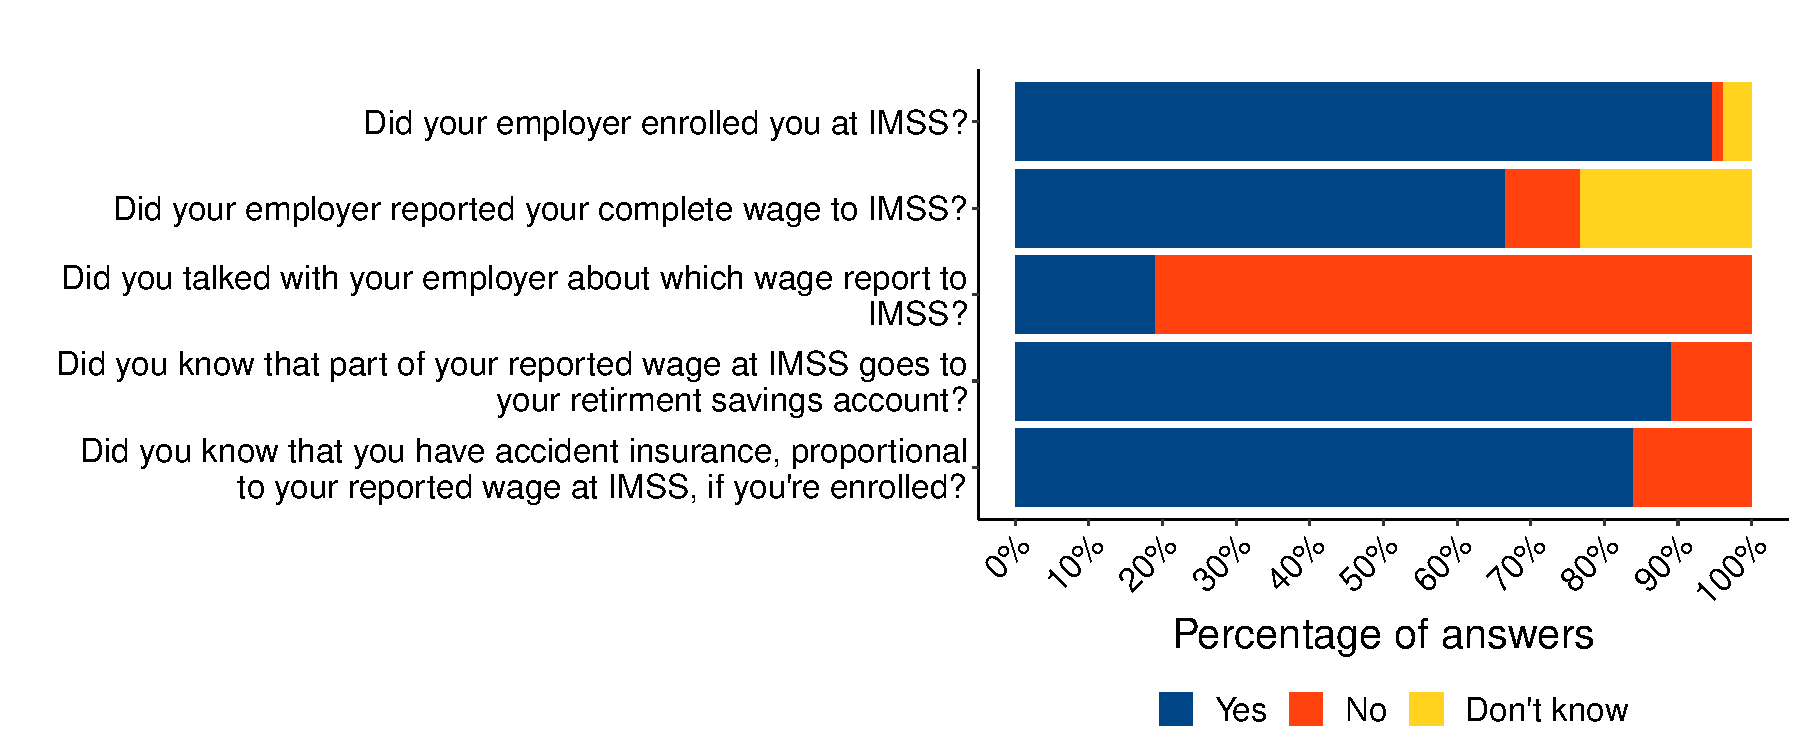
\includegraphics[width=\textwidth]{04_Figures/worker_survey/hist_knowledge_register_survey.pdf}
\end{figure}
\scriptsize{\textit{Notes}: This figure shows answers to questions about IMSS and wage reporting from the worker survey. \textit{Sample:} 233,709 answers from a survey conducted via email to workers enrolled at IMSS during August 2021. Questions 1-2, about the worker's employer, included the option "I don't know". Questions 3-5 ask about the worker's actions or knowledge didn't include the option "I don't know".}

\clearpage

%\subsection{RPCI}

\begin{figure}[H]
    \label{rpci_example}
    \caption{RPCI example}
    \begin{center}
    
    \begin{subfigure}{0.49\textwidth}
    \caption{RPCI within the IMSS Digital app}
    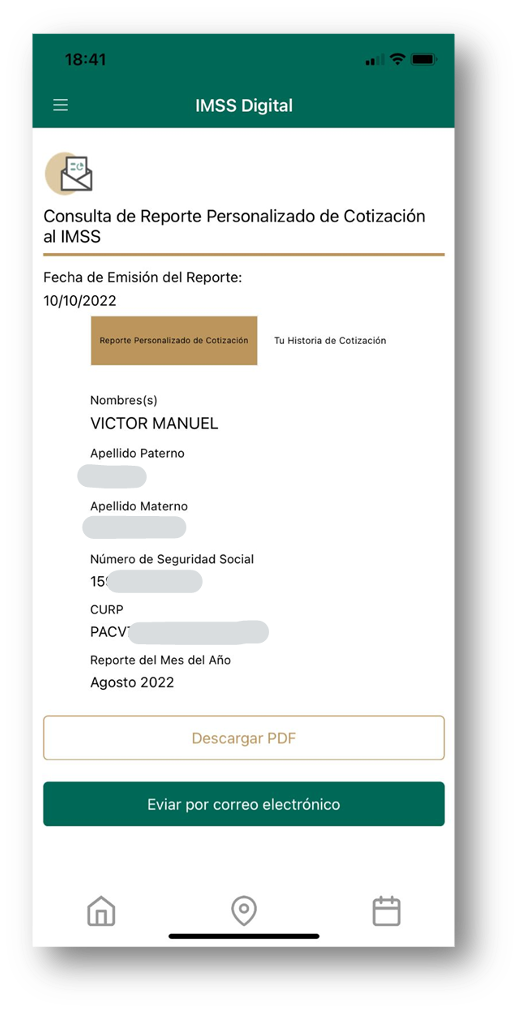
\includegraphics[width=\textwidth]{04_Figures/rpci_app/rpci_2.png}
    \end{subfigure}
    \begin{subfigure}{0.49\textwidth}
    \caption{RPCI PDF file}
    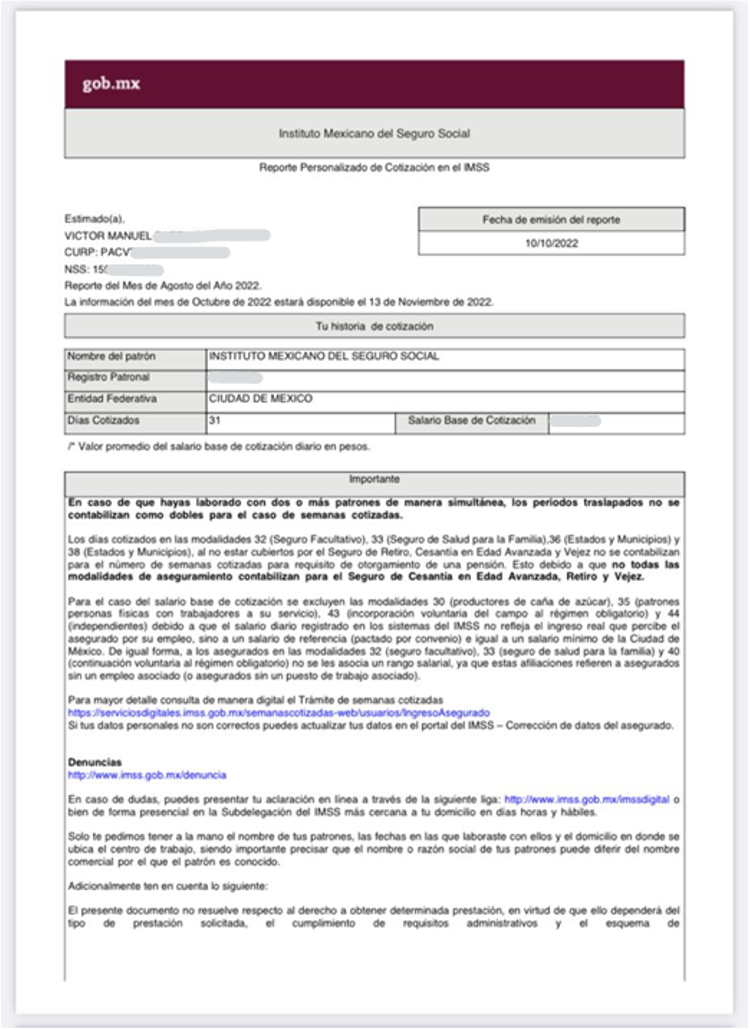
\includegraphics[width=\textwidth]{04_Figures/rpci_app/rpci_3.png}
    \end{subfigure}
    

    \end{center}
\end{figure}
\scriptsize{
\noindent Figure (a) shows the IMSS Digital app, where once the worker is registered for the RPCI, the worker can download their report in PDF or receive it via email. Figure (b) shows an example of the PDF for the RPCI. The report includes the worker job registered information, such as wage and the firm the worker is registered at.
}



%\subsection{RPCI registers by month}

\begin{figure}[H]
    \caption{RPCI registers by month}
    \label{hist_download}
    \begin{center}
    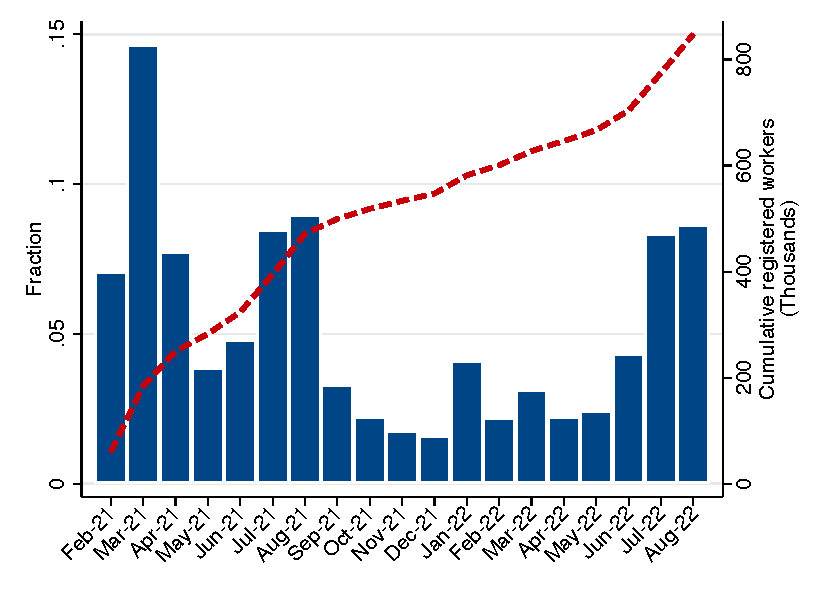
\includegraphics[width=0.65\textwidth]{04_Figures/muestra_1porciento/hist_download_month.pdf}
    \end{center}
\end{figure}
\scriptsize{
\noindent This figure shows the total number of workers registered for the RPCI. The right y-axis measures the fraction of workers who registered for the RPCI during each month from the total workers who registered for the RPCI. The left y-axis measures the cumulative number of workers who registered for the RPCI.
}

\clearpage

%\subsection{Event Studies: RPCI effect on enrollment and wages}

\begin{figure}[H]
    \centering
    \caption{Event studies - RPCI effect on enrollment and wages \label{fig:event_study_rpci}}
    
    \begin{subfigure}{0.49\textwidth}
    \caption{Effect on being enrolled}
    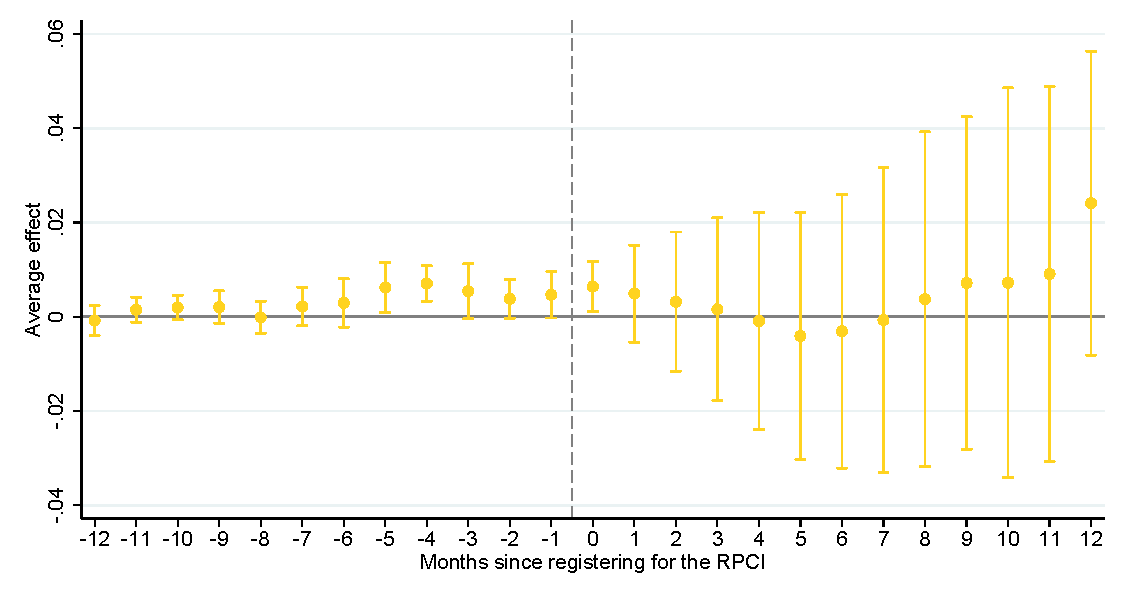
\includegraphics[width=\textwidth]{04_Figures/muestra_10porciento/event_study_alta_dcdh.pdf}
    \end{subfigure}
    
    \begin{subfigure}{0.49\textwidth}
    \caption{Effect on formal wage}
    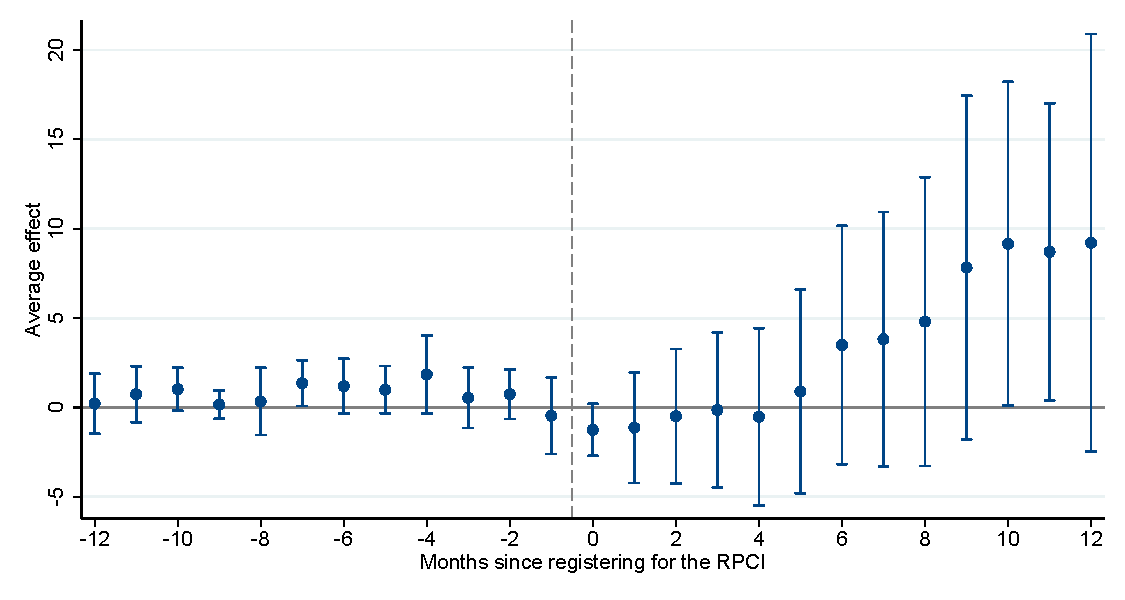
\includegraphics[width=\textwidth]{04_Figures/muestra_10porciento/event_study_sal_formal_dcdh.pdf}
    \end{subfigure}
    \begin{subfigure}{0.49\textwidth}
    \caption{Effect on wage$^\dagger$}
    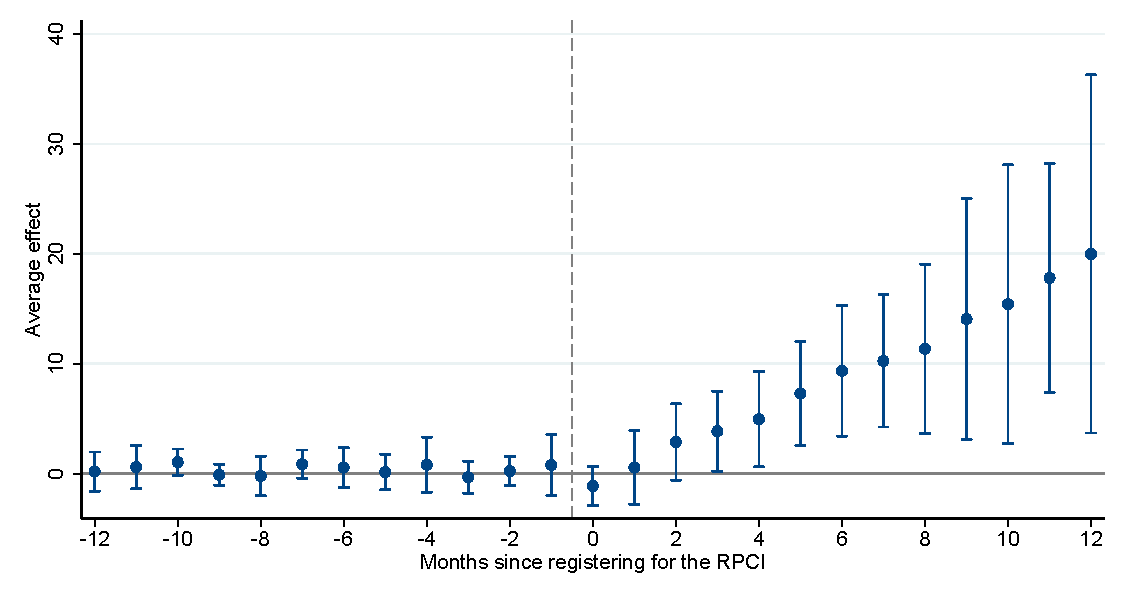
\includegraphics[width=\textwidth]{04_Figures/muestra_10porciento/event_study_sal_cierre_dcdh.pdf}
    \end{subfigure}
    
    %\textit{Do file: event_study_rpci.do}
\end{figure}

\scriptsize{
\noindent \textit{Notes}: This figures shows the event studies for the effect of registering to the RPCI on enrollment and the worker's wage. \textit{Sample:} Panel data for a random sample of the workers enrolled at the Mexican Institute of Social Security (IMSS) during during 2020 and January 2021 (before the RPCI launch). \textit{Enrolled} is a dummy variable where 1 means worker $i$ was enrolled at IMSS during period $t$. $\dagger$ \textit{Formal Wage} and \textit{Wage} are the registered wage for worker $i$ during period $t$, the difference is \textit{Formal Wage} is 0 when the worker isn't enrolled, while \textit{Wage} is missing when the worker isn't enrolled. The event studies follow the estimators proposed by \cite{de2020two}, using the robust dynamic option to account for possible heterogeneous treatment effects across cohorts. Robust standard errors clustered by worker id. This figure is referenced in %\hyperref[subsec:workers]{Section} \ref{subsec:workers}.
}

\clearpage

\begin{comment}
    
%\subsection{Event Studies: RPCI effect on wage changes}

\begin{figure}[H]
    \centering
    \caption{Event studies - RPCI effect on wage changes \label{fig:event_study_wage_changes_rpci}}
    
    \begin{subfigure}{0.49\textwidth}
    \caption{Effect on wage changes}
    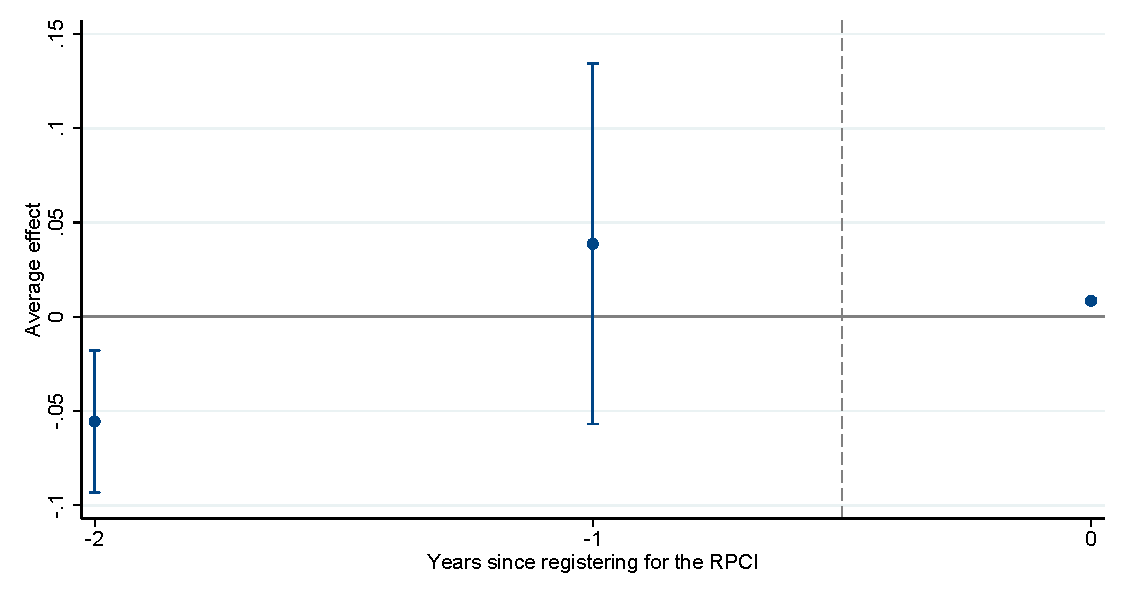
\includegraphics[width=\textwidth]{04_Figures/muestra_10porciento/event_study_sal_diff_yr_dcdh.pdf}
    \end{subfigure}
    
    \begin{subfigure}{0.49\textwidth}
    \caption{Effect on wage raises}
    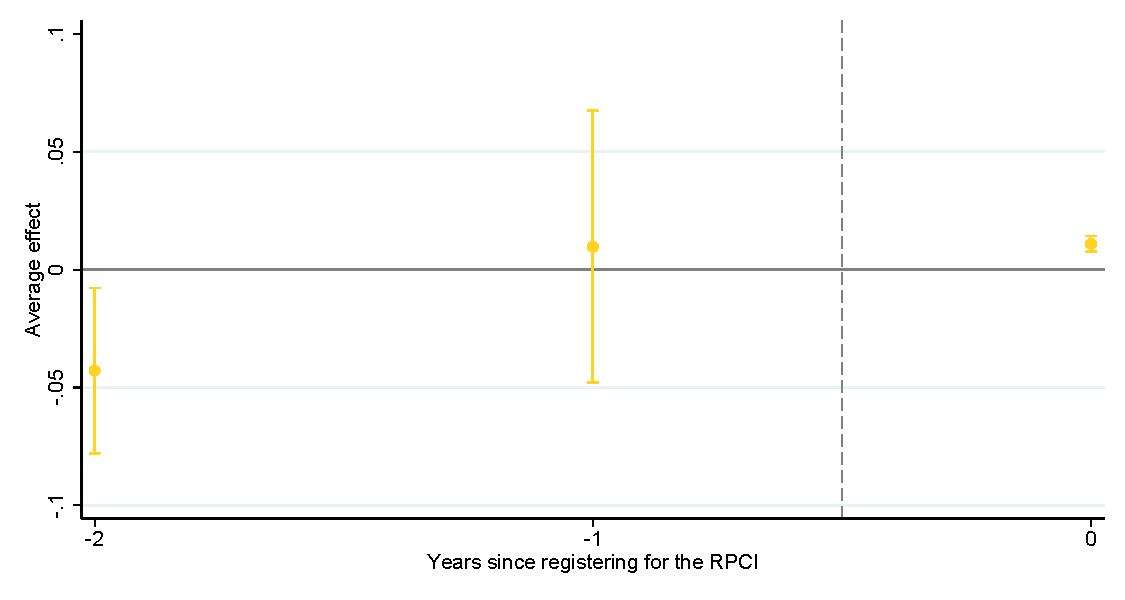
\includegraphics[width=\textwidth]{04_Figures/muestra_10porciento/event_study_sal_mayor_yr_dcdh.pdf}
    \end{subfigure}
    \begin{subfigure}{0.49\textwidth}
    \caption{Effect on wage cuts}
    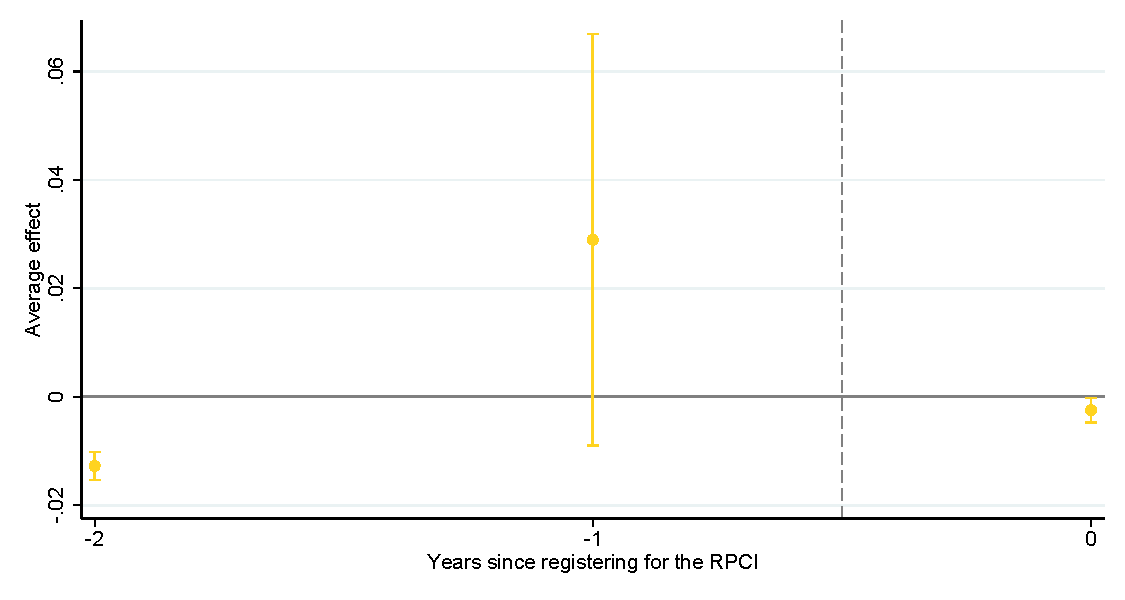
\includegraphics[width=\textwidth]{04_Figures/muestra_10porciento/event_study_sal_menor_yr_dcdh.pdf}
    \end{subfigure}
    
    %\textit{Do file: event_study_rpci.do}
\end{figure}

\scriptsize{
\noindent \textit{Notes}: This figures shows the event studies for the effect of registering to the RPCI on enrollment and the worker's wage. \textit{Sample:} Panel data for a random sample of the workers enrolled at the Mexican Institute of Social Security (IMSS) during during 2020 and January 2021 (before the RPCI launch). \textit{Wage Changes} counts the number of changes in the reported wage at IMSS of worker $i$ during year $t$. \textit{Wage Raises} counts the number of wage changes where the wage increased and \textit{Wage Cuts} counts the number of wage changes where the wage decreased. The event studies follow the estimators proposed by \cite{de2020two}, using the robust dynamic option to account for possible heterogeneous treatment effects across cohorts. Robust standard errors clustered by worker id. This figure is referenced in %\hyperref[subsec:workers]{Section} \ref{subsec:workers}.
}

\end{comment}

%\subsection{Heterogeneity by worker characteristics}

\begin{figure}[H]
    \centering
    \caption{Heterogeneity by worker characteristics \label{fig:heterogeneity_worker_rpci}}
    
    \begin{subfigure}{\textwidth}
    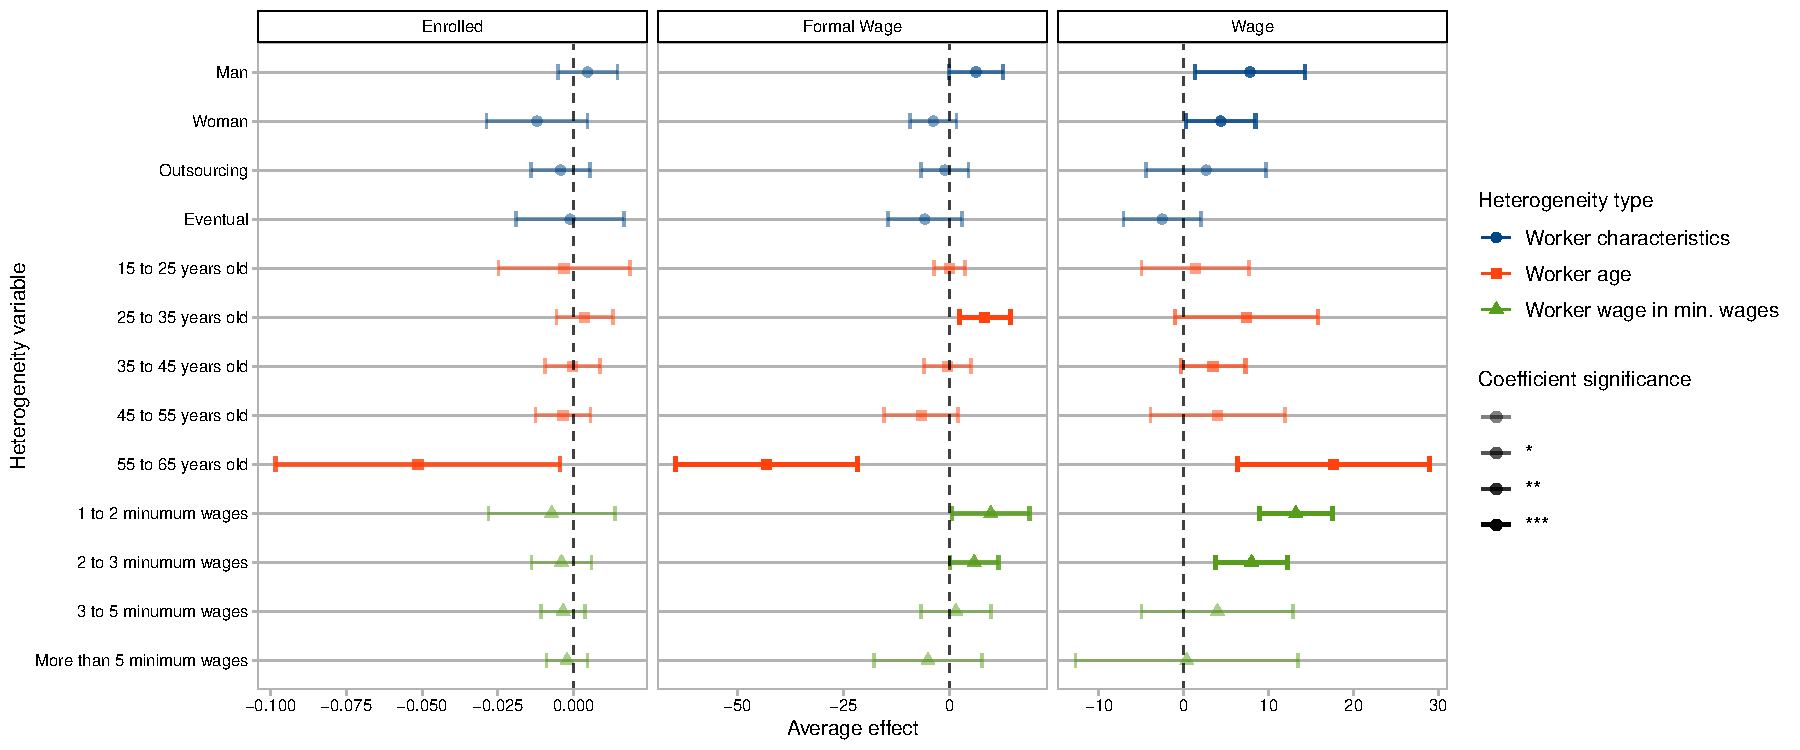
\includegraphics[width=\textwidth]{04_Figures/muestra_10porciento/dcdh_heterogeneity_worker_characteristics_paper.pdf}
    \end{subfigure}
    
    %\textit{Do file: dcdh_heterogeneity_rpci.do}
\end{figure}

\scriptsize{
\noindent \textit{Notes}: This figure explores heterogeneity in the effect of registering to the RPCI on enrollment and the worker's wage by baseline worker's characteristics (characteristics during 2020, before the RPCI launch). \textit{Sample:} Panel data for a random sample of the workers enrolled at the Mexican Institute of Social Security (IMSS) during during 2020 and January 2021 (before the RPCI launch). \textit{Enrolled} is a dummy variable where 1 means worker $i$ was enrolled at IMSS during period $t$. $\dagger$ \textit{Formal Wage} and \textit{Wage} are the registered wage for worker $i$ during period $t$, the difference is \textit{Formal Wage} is 0 when the worker isn't enrolled, while \textit{Wage} is missing when the worker isn't enrolled. The coefficient displayed is the average treatment effect estimated following \cite{de2020two}, using the robust dynamic option to account for possible heterogeneous treatment effects across cohorts. 95\% confidence intervals shown. Robust standard errors clustered by worker id. *** $p<0.01$, ** $p<0.05$, * $p<0.1$. This figure is referenced in %\hyperref[subsec:workers]{Section} \ref{subsec:workers}.
}

\clearpage

%\subsection{Heterogeneity by firm characteristics}

\begin{figure}[H]
    \centering
    \caption{Heterogeneity by firm characteristics \label{fig:heterogeneity_firm_rpci}}
    
    \begin{subfigure}{\textwidth}
    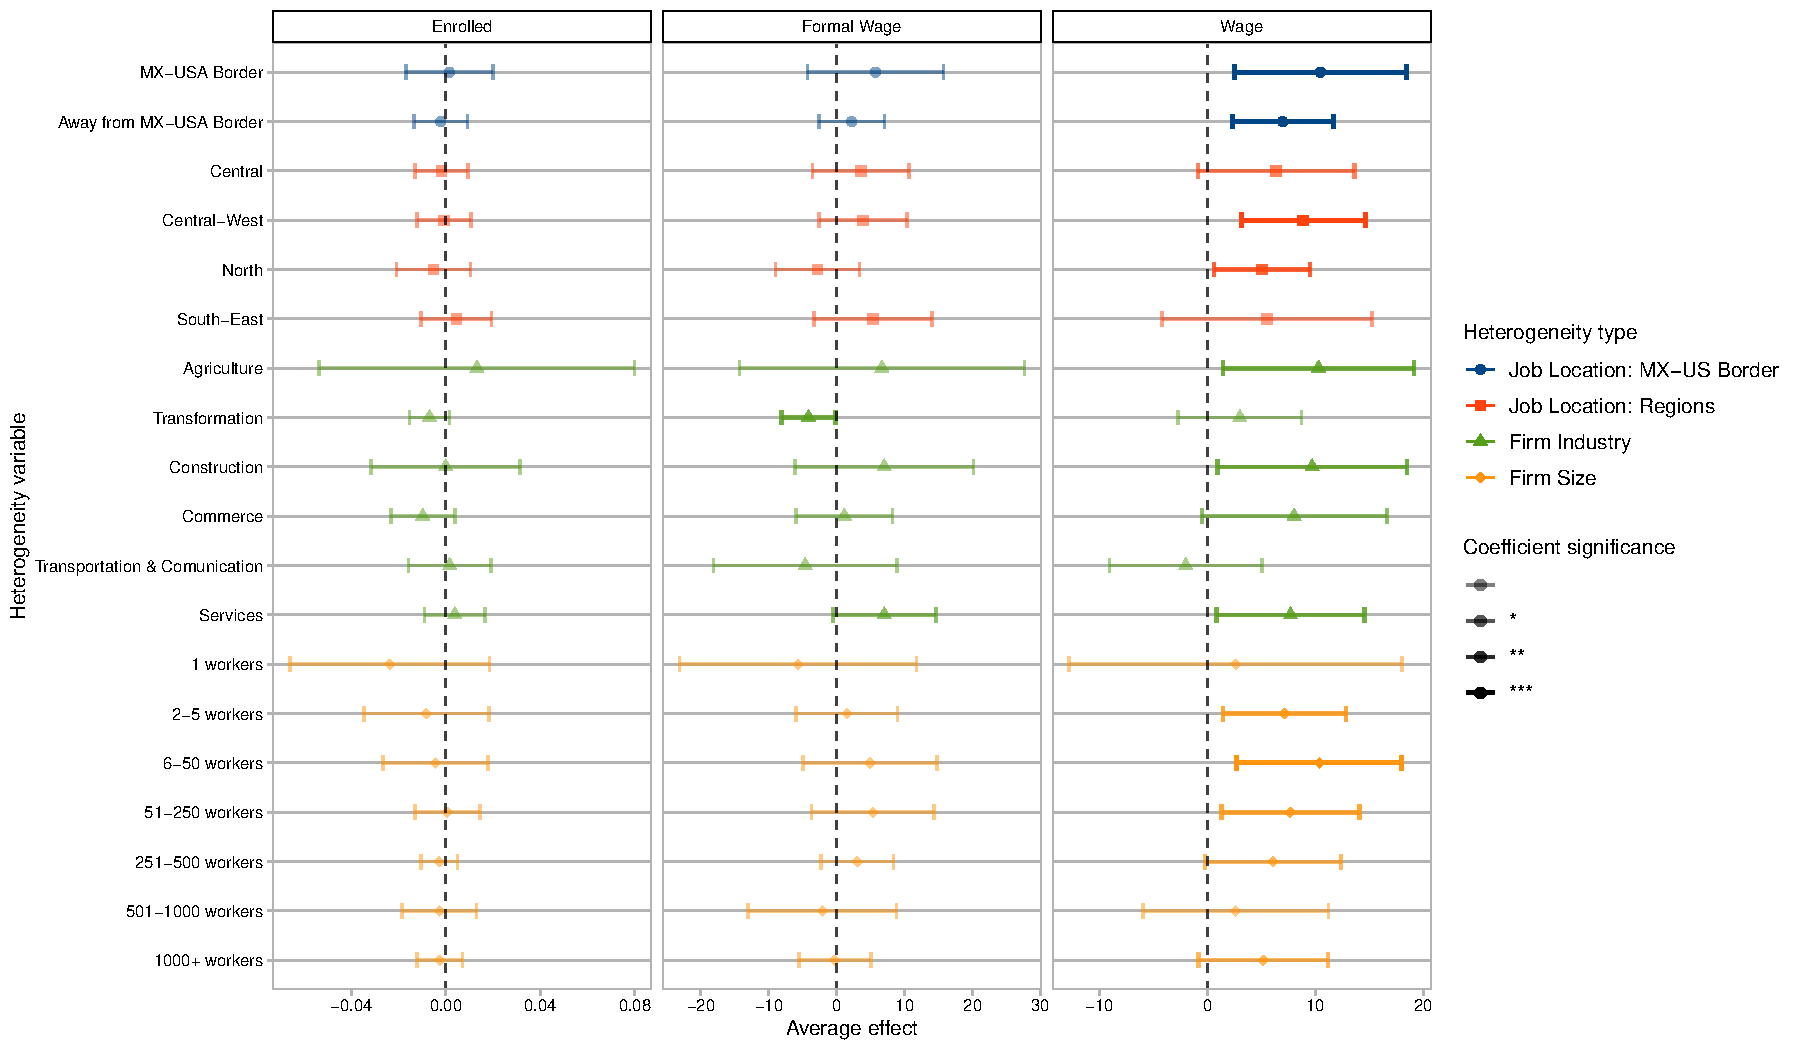
\includegraphics[width=\textwidth]{04_Figures/muestra_10porciento/dcdh_heterogeneity_firm_characteristics_paper.pdf}
    \end{subfigure}
    
    %\textit{Do file: dcdh_heterogeneity_rpci.do}
\end{figure}

\scriptsize{
\noindent \textit{Notes}: This figure explores heterogeneity in the effect of registering to the RPCI on enrollment and the worker's wage by baseline firm's characteristics (characteristics during 2020, before the RPCI launch). \textit{Sample:} Panel data for a random sample of the workers enrolled at the Mexican Institute of Social Security (IMSS) during during 2020 and January 2021 (before the RPCI launch). \textit{Enrolled} is a dummy variable where 1 means worker $i$ was enrolled at IMSS during period $t$. $\dagger$ \textit{Formal Wage} and \textit{Wage} are the registered wage for worker $i$ during period $t$, the difference is \textit{Formal Wage} is 0 when the worker isn't enrolled, while \textit{Wage} is missing when the worker isn't enrolled. The coefficient displayed is the average treatment effect estimated following \cite{de2020two}, using the robust dynamic option to account for possible heterogeneous treatment effects across cohorts. 95\% confidence intervals shown. Robust standard errors clustered by worker id. *** $p<0.01$, ** $p<0.05$, * $p<0.1$. This figure is referenced in %\hyperref[subsec:workers]{Section} \ref{subsec:workers}.
}

\clearpage

%%%%%%%%%%%%%%%%%%%%%%%%%%%%%%%%%%%%%%%%%%%%%%%%%%%%%%

\newpage
%  \documentclass[oneside,11pt]{article}

% 
\usepackage{soul}
\usepackage{natbib}
\usepackage{hyperref}
\usepackage{bookmark}
\usepackage{graphicx}             
\graphicspath{{./Figuras/}}
\usepackage[dvipsnames]{xcolor}
\usepackage{todonotes}
\usepackage{makecell}
\usepackage[margin=1in]{geometry}
\usepackage{float}                
\usepackage{amsmath}
\usepackage{amscd}
\usepackage{amsfonts}
\usepackage{amssymb}
\usepackage{bbm}
\usepackage{booktabs}
\usepackage{nameref}
\usepackage{multirow}
\usepackage[nokeyprefix]{refstyle}
\usepackage{rotating}
\usepackage{threeparttable}
\usepackage{afterpage}
\usepackage{lscape}
\usepackage{enumerate}
\usepackage{caption}
\usepackage{subcaption}
\usepackage{epstopdf}
\usepackage{setspace}
\usepackage{svg}
\usepackage{dsfont}
\usepackage{amsthm}
\usepackage{tocloft}
\usepackage{etoc}
\usepackage{lmodern}
\usepackage{bm}
\usepackage[T1]{fontenc}
\usepackage{tgpagella}

\epstopdfDeclareGraphicsRule{.tiff}{png}{.png}{convert #1 \OutputFile}
\AppendGraphicsExtensions{.tiff}

\epstopdfDeclareGraphicsRule{.tif}{png}{.png}{convert #1 \OutputFile}
\AppendGraphicsExtensions{.tif}

\def\sym#1{\ifmmode^{#1}\else\(^{#1}\)\fi}

\usepackage{tikz}
\usetikzlibrary{shapes.geometric, arrows}
\usetikzlibrary{calc}
\usetikzlibrary{matrix}

\tikzset{ 
    table/.style={
        matrix of nodes,
        row sep=-\pgflinewidth,
        column sep=-\pgflinewidth,
        nodes={
            rectangle,
            draw=black,
            align=center
        },
        minimum height=1.5em,
        text depth=0.5ex,
        text height=2ex,
        nodes in empty cells,
%%
        every even row/.style={
            nodes={fill=gray!20}
        },
        column 1/.style={
            nodes={text width=2em,font=\bfseries}
        },
        row 1/.style={
            nodes={
                fill=black,
                text=white,
                font=\bfseries
            }
        }
    }
}


\usepackage{colortbl}
\usepackage{url}
\urlstyle{rm}
\definecolor{darkblue}{rgb}{0,0,.4}
\hypersetup{colorlinks=true, breaklinks=true, citecolor=Maroon, linkcolor=darkblue, menucolor=darkblue, urlcolor=darkblue}

\newtheorem{theorem}{Theorem}
\newtheorem{claim}[theorem]{Claim}
\newtheorem{prop}[theorem]{Proposition} 
\newtheorem{cor}[theorem]{Corollary} 
\newtheorem{assumption}{Assumption} 
\newtheorem{lem}{Lemma} 

\DeclareRobustCommand{\hlgr}[1]{{\sethlcolor{green}\hl{#1}}}


\usepackage{comment}
%para esconder columnas en tablas (enrique)
\usepackage{array}
\newcolumntype{H}{>{\setbox0=\hbox\bgroup}c<{\egroup}@{}}
\linespread{1.25}

\newcommand{\wh}{\widehat}
\usepackage{anyfontsize}

\usepackage[linesnumbered,vlined,ruled,commentsnumbered]{algorithm2e}

\DontPrintSemicolon
\newcommand{\To}{\mbox{\upshape\bfseries to}}
\newcommand{\E}{\mathbb{E}}

\DeclareCaptionFormat{cont}{#1 (cont.)#2#3\par}
% %%% HELPER CODE FOR DEALING WITH EXTERNAL REFERENCES
% \usepackage{xr}
% \makeatletter
% \newcommand*{\addFileDependency}[1]{
%   \typeout{(#1)}
%   \@addtofilelist{#1}
%   \IfFileExists{#1}{}{\typeout{No file #1.}}
% }
% \makeatother


% \newcommand*{\myexternaldocument}[1]{
%     \externaldocument{#1}
%     \addFileDependency{#1.tex}
%     \addFileDependency{#1.aux}
% }

% %\myexternaldocument{OA}

% %%%%%%%%%%%%%%%%%%%%%%%%%%%%%%%% DOCUMENT
% \begin{document}

%%%%%%%%%%%%%%%%%%%%%%%%%%%%%%%%%%%%%%%%%%%%%%%

% APPENDIX 
\setcounter{table}{0}
\setcounter{figure}{0}
\setcounter{section}{0}
\pagenumbering{gobble}


\begin{center}
	\LARGE IMSS RPCI \\[0.5em]
	\Large{Appendix $-$ For Online Publication} \\[1em]
	\large \author{Eduardo Alcaraz \and Gabriela López \and Luis Martínez \and Marco Medina \and Enrique Seira}
\end{center}

\appendix
\pagenumbering{arabic}
\renewcommand\thefigure{OA-\arabic{figure}}
\renewcommand\thetable{OA-\arabic{table}}
\renewcommand*{\thepage}{OA - \arabic{page}}
\renewcommand\thesection{Appendix \Alph{section}.}
\renewcommand\thesubsection{\Alph{section}.\arabic{subsection}}

%\renewcommand{\cftparskip}{0em} % NOT NEEDED
\renewcommand\cftsecdotsep{\cftdotsep}
\renewcommand\cftsubsecdotsep{\cftnodots}
\renewcommand{\cftsecnumwidth}{6em}
 \renewcommand{\cftpnumalign}{r}
%\renewcommand{\cftsecleader}{\normalfont\cftdotfill{\cftsecdotsep}}


\renewcommand{\cftsecleader}{\cftdotfill{\cftsecdotsep}\hspace{1.8em}}
%\renewcommand{\cftsecpagefont}{20em}
%\renewcommand{\cftfignumwidth}{6em}
%\renewcommand{\cfttabnumwidth}{3.3em}

%\tableofcontents
\etocdepthtag.toc{mtappendix}
\etocsettagdepth{mtchapter}{none}
\etocsettagdepth{mtappendix}{subsection}

\setstretch{0.9}
%\renewcommand\contentsname{} % the empty name

\begingroup
\let\clearpage\relax
%\vspace{-1.5em} % the removed space. Set as appropriate
\tableofcontents
\endgroup

\clearpage

\section{ RPCI}
\vspace{.2in}

\begin{figure}[H]
    \caption{RPCI flyers}
    \label{rpci_flyers}
    \begin{center}
    
    \begin{subfigure}{0.49\textwidth}
    \caption{RPCI flyer titled "Does my employer has me registered at IMSS?"}
    
\includegraphics[width=\textwidth]{04_Figures/rpci_app/rpci_flyer_3.jpeg}
    \end{subfigure}
    \begin{subfigure}{0.49\textwidth}
    \caption{RPCI flyer titled "Digital services for a healthy environment"}
    
\includegraphics[width=\textwidth]{04_Figures/rpci_app/rpci_flyer_2.jpeg}
    \end{subfigure}

    \end{center}
\end{figure}
\scriptsize{
\noindent Flyers circulated by the Mexican Institute of Social Security (IMSS) for the RPCI. Both flyers explain how you can track and access your job register information, such as wage and firm you are registered at, if you register for the RPCI.
}

\clearpage

\begin{figure}[H]
    \caption{Registering for the RPCI}
    \label{rpci_register}
    \begin{center}
    
    \begin{subfigure}{0.9\textwidth}
    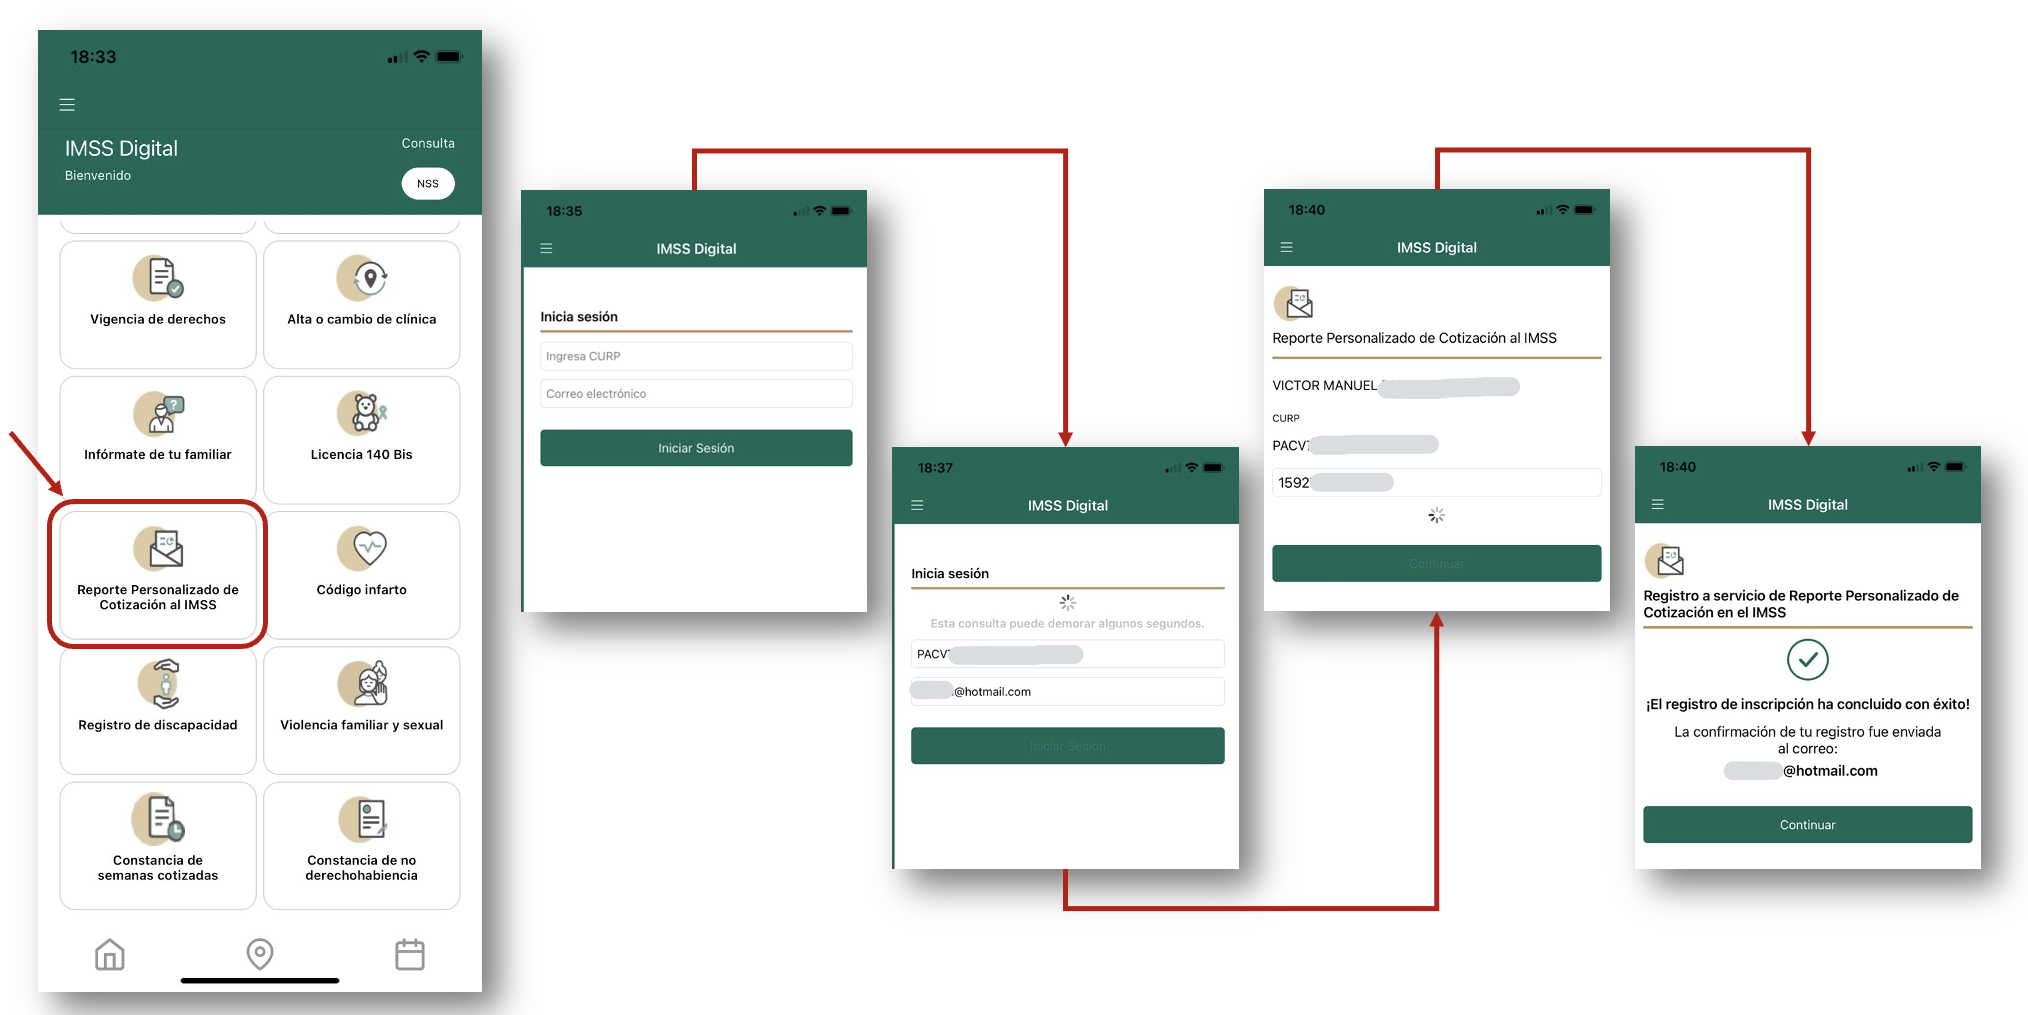
\includegraphics[width=\textwidth]{04_Figures/rpci_app/rpci_register.png}
    \end{subfigure}

    \end{center}
\end{figure}
\scriptsize{
\noindent Diagram shows how to register for the RPCI within the IMSS Digital app. The worker registers only once to access the RPCI, using his Unique Population Registry Key (CURP) and email address.
}

\clearpage

\begin{figure}[H]
    \caption{RPCI example}
    \label{rpci_example}
    \begin{center}
    
    \begin{subfigure}{0.49\textwidth}
    \caption{RPCI within the IMSS Digital app}
    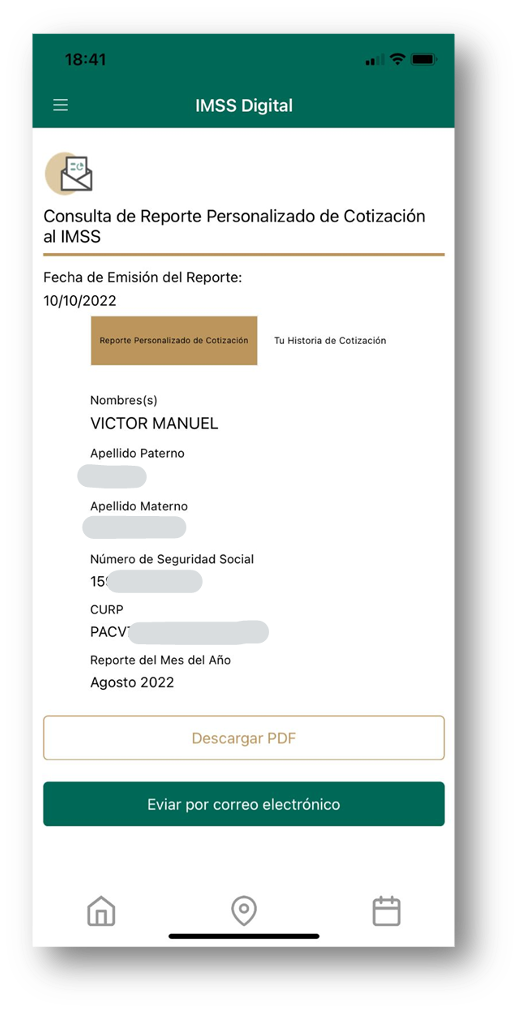
\includegraphics[width=\textwidth]{04_Figures/rpci_app/rpci_2.png}
    \end{subfigure}
    \begin{subfigure}{0.49\textwidth}
    \caption{RPCI PDF file}
    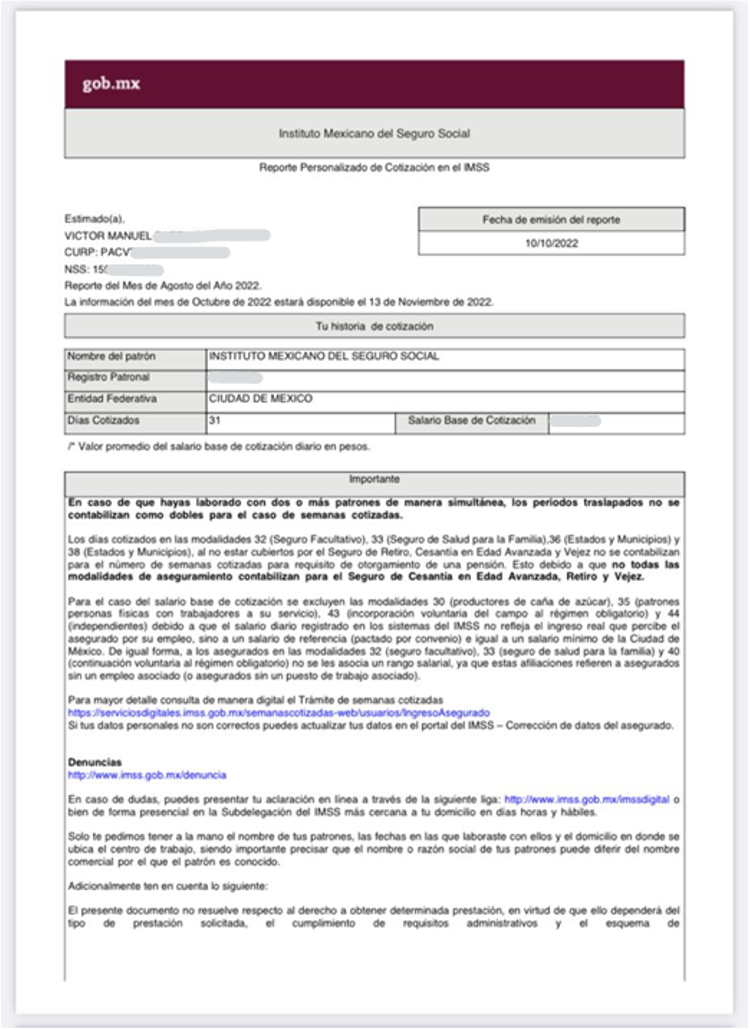
\includegraphics[width=\textwidth]{04_Figures/rpci_app/rpci_3.png}
    \end{subfigure}
    

    \end{center}
\end{figure}
\scriptsize{
\noindent Figure (a) shows the IMSS Digital app, where once the worker is registered for the RPCI, the worker can download their report in PDF or receive it via email. Figure (b) shows an example of the PDF for the RPCI. The report includes the worker job registered information, such as wage and the firm the worker is registered at.
}

%\clearpage

%\bibliographystyle{authordate1}
%\bibliographystyle{amsalpha}
%\bibliographystyle{AER}

%\bibliography{References}




% \end{document}

\end{document}

